\documentclass[a4paper,12pt]{report}

\usepackage[serbian, ngerman, english]{babel}
\usepackage[a4paper, inner=3cm, outer=3cm, top=2cm, bottom=2cm]{geometry}
\usepackage{blindtext}
\usepackage{microtype}
\usepackage{graphicx}
\usepackage{wrapfig}
\usepackage{enumitem}
\usepackage{fancyhdr}
\usepackage{amsmath}
\usepackage{index}
\usepackage[autostyle]{csquotes}
\usepackage{amssymb}
\DeclareMathOperator*{\argmax}{argmax}
\usepackage{listings}
%\usepackage{booktabs}

\makeindex
%after this beguins the document

\begin{document}
\selectlanguage{serbian} 
%\renewcommand{\contentsname}{Sadržaj}
%\renewcommand{\chaptername}{Poglavlje}

\title{\Large{\textbf{Service mesh infrstrukturni sloj distribuiranih aplikacija }}}
\author{Student: Danilo Veljović, broj indeksa: 1120}
\date{Novembar 6, 2020}
\maketitle
\let\cleardoublepage\clearpage
\tableofcontents

\pagenumbering{arabic}

\setcounter{page}{1}

\chapter{Uvod}

Web aplikacije čine veliki deo naše svakodnevice. Preko njih se informišemo, naručujemo stvari, trgujemo, a u ovo vreme ih i sve češće koristimo za rad od kuće. Samim tim i očekivanja korisnika od ovih aplikacija vremenom postaju sve veća. Uz to što aplikacije moraju da podržavaju veliki broj istovremenih korisnika, one moraju biti stalno dostupne, otporne na greške i lake za održavanje i dodavanje novih funkcionalnosti. Kao odgovor na ove potrebe smišljena je \textit{arhitektura mikroservisa} koja je postavila presedan u razvoju softvera i postala defakto standard za savremene aplikacije. U arhitekturi mikroservisa sistem se projektuje kao skup nezavisnih servisa koji implementiraju različite funkcionalnosti i koji mogu međusobno da komuniciraju.  Ovako projektovane aplikacije se mogu lako skalirati kako se broj korisnika povećava, pojedini servisi se mogu nezavisno postavljati na server, pa je lako menjati pojedine delove tako da to ne utiče na ostatak sistema. Ovakvi sistemi su takođe jako otporni na greške, i ako jedan od servisa prestane da funkcioniše, to neće uticati na ostale servise.  \newline

Jedan od glavnih izazova u implementaciji ovakve arhitekture je interservisna komunikacija. Servisi mogu komunicirati međusobom sinhrono ili asinhrono. Ukoliko dođe do gubitka poruka usled komunikacije to može dovesti sistem u neočekivano stanje. Još jedan od problema je skaliranje i postavljanje na server koje se danas sve češće rešava kombinacijom Docker i Kubernetes. Međutim ovo zahteva dodatnu infrastrukturu i inženjere koji su isključivo posvećeni tom delu sistema što može biti jako skupo. Rutiranje takođe može biti problematično u mikroservisnoj arhitekturi. Najčešće se koristi API gateway obrazac za rutiranje zahteva, međutim ovaj jednostavan obrazac sve češće ne može da odgovori na rastuće zahteve sistema. \newline

Kao jedno od rešenja, pre svega infrastrukturnih, problema mikroservisnih sistema, smišljen je \textit{service mesh}. Service mesh (srp. servisna mreža, mreža servisa) je poseban infrastrukturni sloj. Konfigurabilan je, ima malu latentnost i dizajniran je tako da podnese intenzivnu interservisnu komunikaciju. Neke od rešenja koje donosi service mesh su: 

\begin{itemize}
	\item olakšano rutiranje
	\item jednostavnije postavljanje novih instanci na server
	\item jednostavna autorizacija i autentifikacija pri interservisnoj komunikaciji
	\item \textit{load balancing}-a (srp. raspoređivanje opterećenja - obrazac po kome se zahtevi raspoređuju ravnomerno svim dostupnim instancama servisa)
	\item enkripcija komunikacije
	\item \textit{circuit breaker} obrazac (srp. prekidač - obrazac kojim se omogućava servisima koji su oboreni ili zatrpani zahtevima, da se oporave)
\end{itemize}

U narednim poglavljima biće reči o samoj definiciji service mesha, prednostima korišćenja ovog obrasca, i \textit{Consul}-u kao jednoj od implementacija service mesh arhitekture. Nakon toga biće dat primer korišćenja Consul-a na jednoj mikroservisnoj aplikaciji.

\chapter{Service mesh arhitektura}

Service mesh je alat koji pomaže u monitoringu, komunikaciji između servisa i kontrolisanju stanja sistema. To je zasebna infrastrukturna komponenta koja se sastoji iz dve ravni: 
\begin{itemize}
	\item ravan podataka (engl. data plane)
	\item ravan kontrole (engl. control plane)
\end{itemize}

Ravan podataka upravlja komunikacijom između instanci servisa. Kontrolna ravan generiše konfiguraciju i dostavlja je do svih instanci u ravni podataka. Korisnik se na kontrolnu ravan može povezati ili API-jem, terminalom ili grafičkim interfejsom. Pregled najvažnijih komponenti service mesh-a dati su na slici  \ref{fig:service-mesh-topology}. 

\begin{figure}[h]
    \centering
    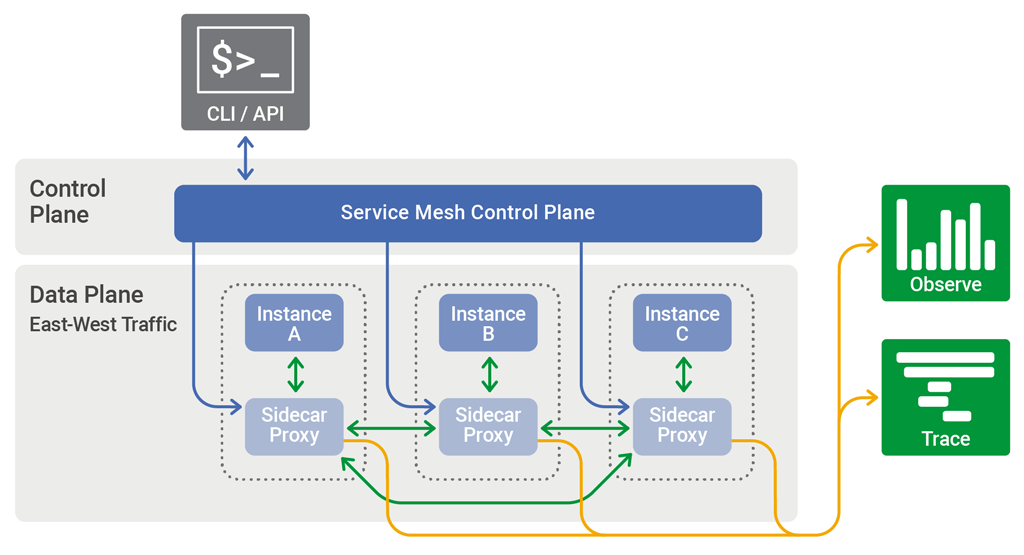
\includegraphics[width=\textwidth]{service-mesh-generic-topology}
    \caption{Service mesh topologija}
    \label{fig:service-mesh-topology}
\end{figure}

U ravni podataka svakoj od deploy-ovanih instanci servisa pridružen je i (jedan ili više) proxy (srp. posrednik). Zajedno, instanca i njen proxy čine sidecar (srp. prikolica) obrazac.  U sidecar obrascu se sve dodatne mogućnosti koje su potrebne servisu, dodaju u proxy-ju koji je zaseban kontejner koji se deploy-a uz aplikaciju. Ovaj obrazac omogućava da se dodaju nove funkcionalnosti bez izmene servisa. Na ovaj način se u service mesh-u dodaju funkcionalnosti poput monitoringa, logovanja, circuit breaker obrasca, load balancinga, enkripcije konekcije itd. Važno je napomenuti da bilo koji saobraćaj prvo prolazi kroz proxy, a zatim dolazi do servisa. Postoji još jedan obrazac koji se ređe koristi za deployment proxy-ja, a to je per-host proxy. U ovom slučaju će svaki host imati svoj proxy. Jedan host može biti virutelna mašina, Kubernetes pod ili poseban server.  \newline

Na primer, ako jedan servis želi da komunicira s drugim servisom, taj zahtev presreće proxy servisa koji šalje zahtev. Proxy rutira zahtev do proxy-ja odredišta. Proxy odredišta presreće pristigli zahtev, pre nego što ga pošalje odredišnom servisu. Korišćenje proxy-ja olakšava da se sva svojstva nevezana za biznis logiku, a koja su zajednička za sve servise smeste u njega. Činjenica da saobraćaj prolazi kroz proxy-je omogućava da se beleži koji servisi međusobno komuniciraju, koliko traje komunikcija, i koliko je potebno da servisi odgovore na zahteve i koji je procenat uspešnosti i nespešnosti zahteva. \newline

Kontrolna ravan služi za centralizovano upravljanje service mesh-om. Bilo kakva promena ponašanja service mesh-a koja se primeni se najpre postavi na kontrolnu ravan i nakon toga kontrolna ravan primenjuje podešavanja na ravan podataka i na proksije. Na slici \ref{fig:service-mesh-topology} se takođe vidi da kontrolna ravan prikuplja i obrađuje telemetrijske podatke. Ovakva arhitektura servis mesha omogućava opcije poput monitoringa, circuit breakinga, canary releasing-a (tehnika kojom se nove promene postepeno uvode sve većem broju korisnika, kako bi se izbegli bug-ovi većih razmera), automatski TLS itd. \newline

Kontrolna ravan može da kontroliše i konfiguriše autorizaciju (koji servis može sa kojim da komunicira) i politiku rutiranja. Ovu konfiguraciju može da postavi korisnik, a onda će kontrolna ravan to proslediti ravni podataka. U ravni podataka se čita tekuća konfiguracija i komunicira se u skladu sa njom. \newline

Nešto malo detaljnija arhitektura service mesh-a je data na slici \ref{fig:advanced-service-mesh-topology}.

\begin{figure}[h]
    \centering
    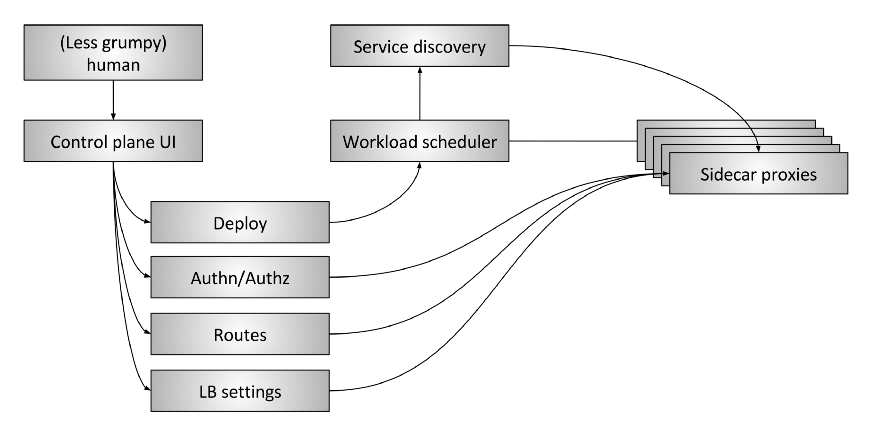
\includegraphics[width=\textwidth]{advanced-service-mesh-architecture}
    \caption{Detaljnija service mesh arhitektura}
    \label{fig:advanced-service-mesh-topology}
\end{figure}

Na slici \ref{advanced-service-mesh-topology} su prikazane sledeće komponente service mesh sistema: 

\begin{itemize}
	\item čovek (engl. the human) - deo sistema koji donosi odluke visokog nivoa, vezane za rutiranje, autorizaciju itd. 
	\item UI ravni kontrole (engl. control plane UI) - čovek/korisnik interaguje sa korisničkim interfejsom kontrolne ravni (bilo da je to web UI, terminal itd). Kroz korisnički interfejs podešava se globalna konfiguracija sistema. Postavke deploymenta (blue/green i/ili preusmerenje saobraćaja), autentifikacija i autorizacija, tabela rutiranja, i postavke load balancinga (npr tajmauti, retries, circuit breakers itd).
	\item Workload scheduler - Servisi se postavljaju na servis mesh pomoću nekog scheduling sistema (npr. Nomad ili Kubernetes). Scheduling sistem je odgovoran za vezivanje servisa sa njegovim proxy-jem.
	\item Service discovery - Kako scheduler postavlja i gasi instance servisa, on to prijavljuje u service discovery sistem. 
\end{itemize}


\chapter{Svojstva service mesh arhitektura}

Sva svojstva service mesh arhitektura se mogu svrstati u jednu od tri kategorije:

\begin{enumerate}
	\item Upravljanje saobraćajem u sistemu
	\item Monitoring/nadgledanje sistema
	\item Bezbednost sistema
\end{enumerate}

Ova svojstva service mesh arhitektura čine ujedno su ujedno i njene prednosti. Korisnik ne mora da brine o tome kako da implementira sve ove funkcionalnosti, jer su one već implementirane za njega. On ima slobodu da podešava već postojeća svojstva i da time podiže stepen bezbednosti u sistemu, uključuje ili isključuje logovanje itd. 

\section{Upravljanje saobraćajem u sistemu}

Service mesh ima mogućnost da upravlja saobraćajem na mreži. Pri tom se uvode mnoga svojstva poput rutiranja, rate limiting (srp. ograničenje broja zahteva po servisu),  circuit breaking i tehnika mirroring. Kod service mesha se konfiguracija specificira na sedmom sloju OSI modela, aplikativnom sloju. Razdvajanje saobraćaja od infrastrukture, stavlja saobraćaj u nadležnost aplikacije i ljudi koji je održavaju. Vlasnici aplikacije i inženjeri najbolje razumeju potrebe aplikacije i prema tome mogu da podešavaju mrežne parametre kod aplikacije. \newline

\textbf{Pouzdana komunikacija}\newline

Service mesh osigurava pouzdanu mrežnu komunikaciju. Greške u komunikaciji se automatski rešavaju na transparentan način. U konfiguraciji se može navesti broj ponovnih pokušaja koji se može načiniti i timeout (vreme na koje se čeka na odgovor, nakon isteka tog vremena zahtev se smatra odbijenim). Slanje zahteva, čekanje i ponovno  Servis koji šalje zahtev svu komunikaciju prepušta proxy-ju. Taj proxy zatim šalje zahtev i čeka na odgovor. Ako odgovor ne dobije nakon timeout intervala, pokušava ponovo. Ako nakon zadatog broja pokušaja ne dobije odgovor, smatra da je servis nedostupan.  Na ovaj način se sva logika oko pouzdanosti prebacuje na proxy, dok se kod servisa ne treba menjati. \newline

\textbf{Circuit breaking}\newline

Ponovno slanje zahteva povećava pouzdanost sistema, međutim povećava i broj zahteva koje prima ciljni servis. Zbog ovoga će opterećenje ciljnog servisa biti veće i servis može postati nestabilan. Za rešavanje ovakvog problema uveo se circuit breaker. Ako je neki servis nedostupan on obično odgovara 503 zahtevom. U service meshu se može postaviti prag za broj ovakvih odgovora koji se mogu primiti. Nakon što se prag pređe, proxy izbacuje ovaj servis iz load balancer poola (load balancer pool - skup instanci servisa koje su dostupne). Novi zahtevi se neće rutirati ka "nezdravim" instancama. Najčešće se circuit breaker implementira tako što se navede maksimalni broj konkurentnih TCP konekcija i otvorenih HTTP zahteva. \newline

\textbf{Rate limiting}\newline

Rate limiting je povezan sa circuit breaking-om. Ta funkcionalnost omogućava da se ograniče zahtevi koji zadovoljavaju određeni kriterijum. To omogućava da se određeni zahtevi ne koriste previše. Ova funkcionalnost je slična otvorenim/javnim API-jevima koji kreću da se "guše" nakon što se pređe određen broj zahteva. Definisanjem rate limita zahteva da se definiše parametar koji se broji, maksimalna vrednost i vremenski prozor u kome se broji taj parametar. Broj zahteva se broji centralizovano tako da ceo sistem ima predstavu koliko zahteva je primljeno. Pažljiva konfiguracija rate limita će osigurati da svi korisnici imaju fer pristup servisu. \newline

\textbf{A/B testiranje}\newline

Upravljanje saobraćajem u service meshu omogućava A/B testiranje. Kada se testira web aplikacija, vlasnici aplikacije mogu da testiraju nove funkcionalnosti, tako što se deo saobraćaja rutira ka instancama servisa koje sadrže nove funkcionalnosti. Onda se može posmatrati telemetrije i da se proučava interakcija korisnika i funkcionalnosti. Iz te interakcije se mogu izvući zaključci da li se korisnicima više sviđa nova funkcionalnost ili stara, da li im se više sviđa jedna implementacija ili neka druga. Čest use-case za A/B testiranje mikroservisa je da se nove funkcionalnosti testiraju samo za ljude iz jednog regiona ili iz neke posebne grupe, ili da se neko ažuriranje proba na manjoj grupi korisnika, pre nego što se pusti svima. Uvek je moguće da se vrati prethodna verzija sistema ako se detektuje previše grešaka u novoj verziji servisa. Ako testiranje novih funkcionalnosti A/B testiranjem može negativno da utiče na sistem, preporučuje se da se koristi canary release.\newline

\textbf{Canary release}\newline

\begin{figure}[h]
    \centering
    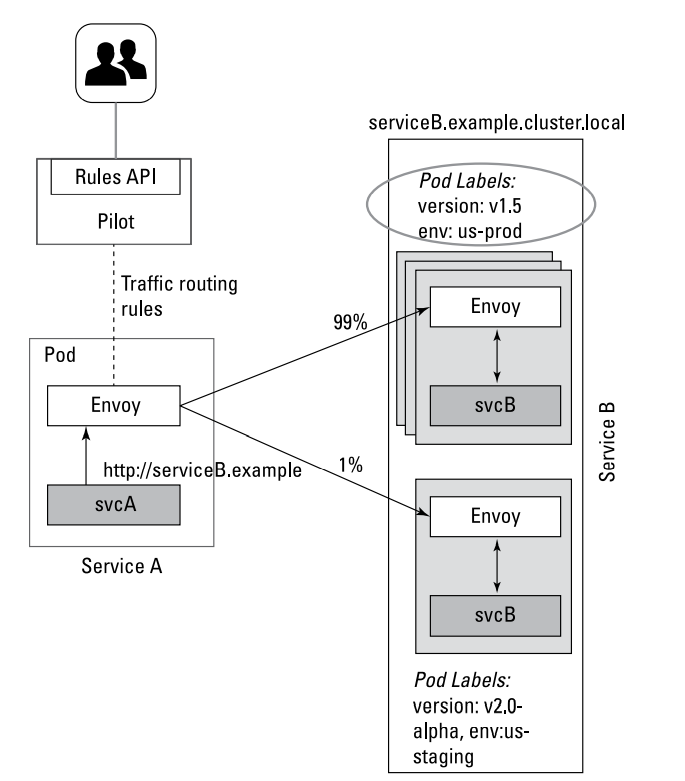
\includegraphics[width=0.5\textwidth]{canary_release_example}
    \caption{Primer Canary release-a}
    \label{fig:canary-release-example}
\end{figure}

Canary release je poseban slučaj A/B testiranja. Kod canary release se mnogo postepenije dešava zamena novih i starih replika. Početna faza kod canary release-a je tzv tamna faza. U ovoj fazi se novom servisu ne prosleđuje saobraćaj. Ako servis je servis "zdrav" vrlo mali procenat saobraćaja se rutira ka njemu (npr 1\%). Motri se na eventualne greške koje se mogu desiti. Sve dok je instanca zdrava, i dok nema grešaka, prosleđuje joj se sve više saobraćaja. Saobraćaj se prosleđuje postepeno, sve dok se 100\% ne bude usmereno ka novim instancama, a stare se postepeno isključuju. Na slici \ref{fig:canary-release-example} je dat primer canary release-a. U tom primeru se 99\% saobraćaja se usmerava ka verziji 1.5, a 1\% saobraćaja se usmerava ka 2.0 verziji. \newline

\textbf{Rutiranje}\newline

Rutiranje/upravljanje saobraćajem omogućava administratorima sistema da kontrolišu tok saobraćaja u aplikaciji. Pravilima rutiranja se određuje da li se može i gde pristigli saobraćaj proslediti na osnovu određenih osobina koji se prosleđuju u HTTP zaglavlju. Na primer, za komunikaciju između dva servisa je vrlo često potrebna neka vrsta autentikacije. Zato servis koji šalje zahtev stavlja u zaglavlje zahteva neki token koji će ga autentifikovati. Kada primajući proxy dobije zahtev, on vidi token za autentifikaciju, i ako je validan dopušta da zahtev stigne do instance. Ovim se eliminiše potreba da autentifikacija bude deo logike sistema, već se jednostavno navodi kao skup pravila u service meshu. Slično se može uraditi i sa lokacijom ili device-om koji šalje poruku. Npr deo saobraćaja se može rutirati, na osnovu lokacije/uređaja sa kojeg dolazi, ka određenom servisu.\newline

Na slici \ref{fig:routing-example} je dat prikaz rutiranja u service meshu. Na gornjoj polovini slike se svi zahtevi rutiraju iz servisa A ka servisu B. Canary release-om se uvodi novi servis za iPhone korisnike. Nakon promene politike rutiranja zahtevi se dele na one koji dolaze od Android uređaja i oni se i dalje rutiranju ka starim instancama servisa B, i zahteve koji dolaze od iPhone uređaja koji se rutiraju ka novoj instanci servisa B. \newline

\begin{figure}[h]
    \centering
    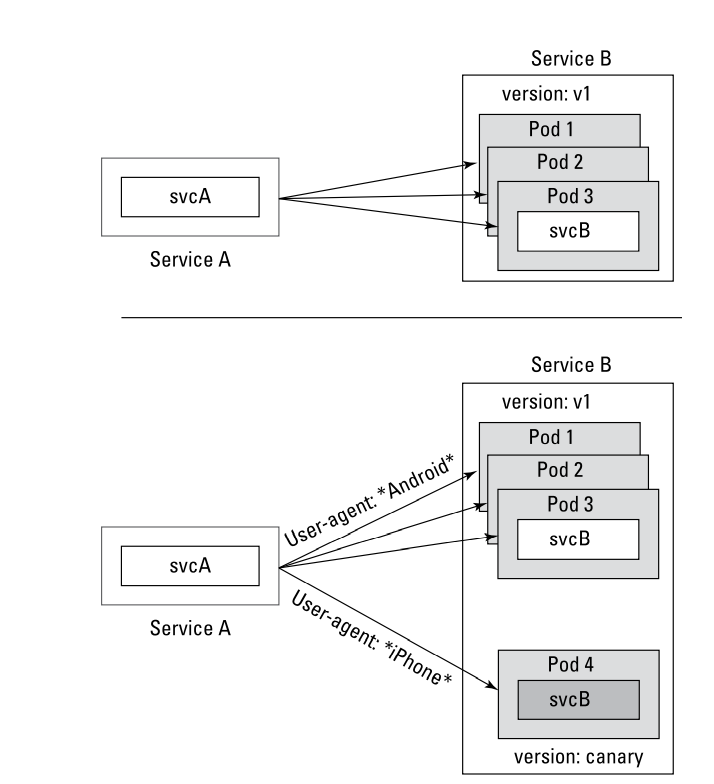
\includegraphics[width=0.7\textwidth]{routing_example}
    \caption{Primer rutiranja u service meshu}
    \label{fig:routing-example}
\end{figure} 

\textbf{Upravljanje spoljnim zahtevima}\newline

Service mesh, podrazumevano, ne dozvoljava spoljne konekcije ka servisima. Međutim, postoji način da se dozvole spoljne konekcije ka određenim URL-ovima. Kontrolisanje saobraćaja koji dolazi preko URL-ova pruža veći stepen fleksibilnosti od korišćenja firewall-a koji koriste IP adresu da filtriraju saobraćaj. Ovo je posledica toga da se IP adresa cloud aplikacije može lako menjati i nije fiksna. Jedan primer je mikroservisna aplikacija koja čita i piše u bazi. Baza je hostovana na javnom cloud-u van service mesha, bez statičke IP adrese. Izlazni saobraćaj mora da bude tako konfigurisan da mikroservisna aplikacija može da se poveže sa bazom koja je van mesha. Jedan pristup bi bio da se whitelist-uje ceo niz IP adresa koje koristi cloud provider. Ovakav pristup dovodi do mogućih bezbednosnih rizika. Sigurniji prilaz bi bio da se kreira poseban proxy - izlazni gateway (engl. egress gateway). Kroz ovaj gateway mora da prođe sav saobraćaj koji napušta service mesh. Korišćenje gateway-a pruža dodatnu kontrolu i može se koristiti Kubernetes za dodatno pooštravanje saobraćaja, tako da se onemogući da bilo koji izlazni saobraćaj, sem onog koji dolazi iz gateway-a, može da napusti klaster. \newline

\begin{figure}[h]
    \centering
    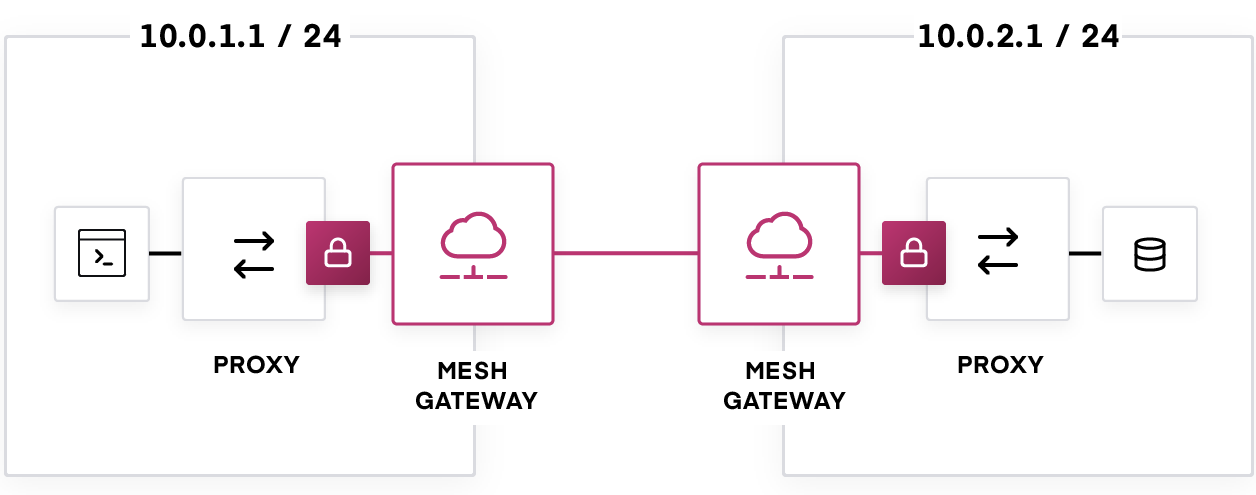
\includegraphics[width=0.7\textwidth]{egress_gateway_example}
    \caption{Primer komunikacije dva klastera preko izlaznog gatewaya}
    \label{fig:egress-gateway-example}
\end{figure} 

Na slici \ref{fig:egress-gateway-example} je dat primer komunikacije dva klastera preko izlaznog gateway-a. Na slici se vidi da se  aplikacija i njena baza nalaze na različitim mrežama. Ako aplikacija želi da komunicira sa bazom, mora da uputi zahtev na URL baze. Taj zahtev prolazi kroz proxy i na osnovu URL-a, proxy prosleđuje zahtev izlaznom gateway-u. Izlazni gateway zatim šalje zahtev na mrežu. Service mesh koji sadrži bazu prima zahtev preko svog izlaznog gateway-a. On se zatim rutira do odgovarajućeg proxy-ja i zatim stiže do servisa kom je bio namenjen. \newline

\section{Nadgledanje sistema}

\textbf{Monitoring}\newline

Mikroservisni sistem treba da uključuje i infrastrukturu za monitoring, koja će prikupljati informacije iz svih mikroservisa i omogućiti svima pristup tim informacijama. Ovo je neophodno da bi se motrilo na metrike velikog broja mikroservisa. Na osnovu ovih metrika se mogu implementirati alarmi ili da se rade dodatne analiza na osnovu ovih metrika. Proxy-ji u ravni podataka, mogu da mere osnovne informacije o mrežnom saobraćaju, kao što su latentnost i propusnost. Moguće je pored ovih informacija izvući još neke dodatne. Service mesh može da razume protokol i da ga tumači. Npr, HTTP protokol ima neki definisan statusni kod koji omogućava service mesh-u da "/ shvati "/ da li je zahtev bio uspešan ili ne. Na ovom osnovu, service mesh može da meri procenat uspešnosti i neuspešnosti zahteva.  Monitoring na nivou service mesh-a ima sledeće prednosti: 

\begin{itemize}
	\item Nema uticaja na kod mikroservisa. Metrike se mere samo u proxy-ju, tako da će svi mikroservisi meriti iste metrike, bez obzira u kom programskom jeziku su pisani ili koji framework koriste.
	\item Metrike daju na uvid stanje mikroservisa. Metrike pokazuju performanse i pouzdanost servisa, koje su korisne krajnjem korisniku i administratoru sistema. Ove metrike su dovoljne da se osigura očekivani kvalitet i pouzdanost servisa. 
\end{itemize}

Metrike koje pruža service mesh su dovoljne za održavanje mikroservisnog sistema. Ali za dublju analizu uzorka problema, potrebne su dodatne metrike koje dolaze iz servisa. U tom slučaju, service mesh takođe može biti od pomoći jer pruža standardizovano okruženje za monitoring, koje service mesh već koristi za svoje metrike. \newline

\textbf{Distribuirano trasiranje}\newline

Trasiranje rešava čest problem u mikroservisnim sistemima. Zahtev ka mikroservisu može za posledicu imati jedan ili više zahteva ka drugim servisima. Trasiranje omogućava praćenje ovakvih zahteva, time olakšavajući nalaženje srži nekog problema. Proxy-ji presreću svaki od zahteva. Međutim da bi bilo moguće raditi trasiranje, treba zaključiti koji zahtev je dolazni, a koji izlazni zahtev. Ovo se obično radi unutar servisa. Obično savaki od servisa ima nekakav jedinstveni ID u sebi, i ova informacija se zatim prosleđuje svim zahtevima koji nastaju od njega. Podaci o svakom zahtevu se  zatim čuvaju u service meshu. Jedinstveni ID nije samo koristan za trasiranje, već se koristi i pri logovanju i može biti jako koristan za praćenje zahteva u servisima. Trasiranje se obično koristi u vrlo specifičnim situacijama, gde je vrlo složena komunikacija između servisa. U većini slučajeva se analiza grešaka može izvršiti samo gledanjem u jedan od servisa, smatrajući ostale crnim kutijama. Podacima prikupljenim trasiranjem se mogu kreirati grafovi zavisnosti. koji ukazuju na to koji servisi međusobno komuniciraju. \newline

\textbf{Logovanje}\newline

Logovanje je još jedan način da se stekne uvid u funkcionisanje mikroservisnog sistema. Service mesh prikuplja informacije o mrežnoj komunikaciji. Te informacije može da piše u log fajl. Pristupni logovi koji sadrže unose za HTTP pristup su važni izvor informacija o radu web aplikacije. Često se log fajlovi koriste za analizu grešaka u mikroservisnom sistemu. Da bi se to uradilo, log fajlovi moraju da imaju detaljne informacije. Mikroservisi moraju sami da loguju tu informaciju. Slično kao kod trasiranja i ovo zahteva promenu načina funkcionisanja servisa. Automatski logovi service mesh-a daju samo informacije o komunikaciji, i primljenim porukama što obično nije od značaja. Prednost Logovanje kod service mesh-eva je ta da programeri ne moraju uopšte da se bave logovanjem. Logovi su uniformni bez obzira na tehnologiju i način logovanja. Čak i ovakvi logovi mogu pomoći prilikom traženja grešaka. \newline
 
\section{Bezbednost sistema}

\chapter{Consul kao primer service mesh}

\chapter{Zaključak}

\end{document}